%\ctparttext{\color{black}\begin{center}
%		Esta es una descripción de la parte de informática.
%\end{center}}

%\part{Parte de informática}
\chapter{Herramientas básicas}

En esta sección se presentarán algunos conceptos y herramientas básicas que nos resultarán útiles a lo largo de los siguientes capítulos.

\section{Ecuaciones en diferencias}

Comenzamos presentando la teoría básica necesaria. Para su elaboración se ha usado principalmente \cite{salinelliDiscreteDynamicalModels2014}.

\begin{definition}
Se define una \textbf{ecuación en diferencias de orden $k$}, con $k\geq 1$, como una ecuación en la que intervienen un número fijo de términos consecutivos de una sucesión.

\begin{equation}
\label{def_ec_diferencias}
F(n,X_n, X_{n+1}, \cdots , X_{n+k}) = 0, \quad \forall n\in\mathbb{N},
\end{equation}


donde $F$ es una función de $k+2$ variables en la forma $F:\mathbb{N}\times I^{k+1}\rightarrow \mathbb{R}$, con $I$ un intervalo con al menos dos puntos, $k$ indica el número de términos necesarios para generar el siguiente y donde la sucesión $\{X_n\}_{n\geq 0}$ es la incógnita.
\end{definition}

En las aplicaciones reales de ecuaciones en diferencias, el subíndice $n$ suele considerarse el tiempo, por lo que en estas se considera positivo y discreto.

\begin{definition}
Una ecuación en diferencias de orden $k$, con $k\geq 1$ se dice que está en \textbf{forma normal} si está expresada de la forma:

\begin{equation}
\label{def_ec_forma_normal}
X_{n+k} = \Phi (n, X_n, X_{n+1}\cdots , X_{n+k-1})
\end{equation}


donde $\Phi$ es una función dada definida en $\Phi :\mathbb{N}\times I^{k}\rightarrow I$.
\end{definition}

\begin{definition}
Una \textbf{solución de una ecuación en diferencias} de orden $k$ es una sucesión $\{X_n\}_{n\geq 0}$ de números reales definida explícitamente de la forma:

$$X_n = f(n),\quad n\geq 0,$$

donde $f: \mathbb{N} \rightarrow I$ es una función que cumple (\ref{def_ec_diferencias}) al sustituir $\{X_n\}_{n\geq 0}$ por $f(n)$ para cualquier $n\in\mathbb{N}$.

El conjunto de todas las soluciones de (\ref{def_ec_diferencias}) se llama \textbf{solución general} de la ecuación.
\end{definition}

\begin{theorem}[Existencia y unicidad]
Sea $\Phi$ una función de la forma presentada en (\ref{def_ec_forma_normal}). Entonces la ecuación en diferencias en forma normal (\ref{def_ec_forma_normal}) tiene solución.
Para cada k-upla $(\alpha_0, \alpha_1, \cdots ,\alpha_{k-1})\in I^{k}$ el problema anterior en forma normal con condiciones iniciales dadas tiene una única solución.

\begin{equation}
\begin{aligned}
X_{n+k} = \Phi (n, X_n, X_{n+1}\cdots , X_{n+k-1}) \\
X_0 = \alpha_0, X_1=\alpha_1, \cdots X_{k-1}=\alpha_{k-1}.
\end {aligned}
\end{equation}

\end{theorem}
\begin{proof}
Sustituyendo las condiciones iniciales en (\ref{def_ec_forma_normal}) con $k=0$ obtenemos el valor exacto para $X_k$, al que llamamos $\alpha_k$. Por definición de $\Phi$, $(\alpha_1, \alpha_2, \cdots ,\alpha_{k})\in I^{k}$, luego sustituyendo de nuevo en la misma ecuación por las condiciones iniciales

$$X_1 = \alpha_1, X_2=\alpha_2, \cdots , X_{k}=\alpha_{k},$$

obtenemos $X_{k+1}$. Repitiendo este proceso se crea una sucesión $\{X_n\}_{n\geq 0}$ única, que es solución de (\ref{def_ec_forma_normal}).
\end{proof}


\subsection{Sistemas de ecuaciones en diferencias}

\begin{definition}
Se define un \textbf{sistema de $m$ ecuaciones en diferencias} como un conjunto de $m$ ecuaciones en diferencias a resolver.

\begin{equation}
\begin{cases}
X_{n+k}^1 = \Phi_1(n, X_n^1, \cdots , X_{n+k-1}^1, X_{n}^2, \cdots , X_{n+k-1}^2, \cdots , X_{n}^m, \cdots X_{n+k-1}^m) \\
\cdots \\
X_{n+k}^m = \Phi_m(n, X_n^1, \cdots , X_{n+k-1}^1, X_{n}^2, \cdots , X_{n+k-1}^2, \cdots , X_{n}^m, \cdots X_{n+k-1}^m)
\end{cases}
\end{equation}

Donde $\Phi_i : \mathbb{N}\times D \rightarrow D$, con $D\subset \mathbb{R}^{mk}$ para todo $i=1,\cdots , m$.

Renombrando, podemos expresar el conjunto de sucesiones como:

\begin{equation}
X_n = (X_{n}^1, X_{n}^2, \cdots , X_{n}^m)^{T}
\end{equation}

luego el sistema de ecuaciones resultaría:

\begin{equation}
\label{def_sist_ec}
X_{n+k} = \Phi (n, X_n, \cdots , X_{n+k-1})
\end{equation}


donde $\Phi : D \rightarrow D$, con $D$ siendo el dominio de la función $\Phi$, y por tanto $D\subset \mathbb{N}\times\mathbb{R}^k$ y con $\Phi = (\Phi_1, \cdots \Phi_m)$.

\end{definition}

\begin{definition}
Una \textbf{solución} de un sistema de ecuaciones en diferencias son las soluciones explícitas de cada ecuación del sistema, de forma que se satisfagan todas ellas; es decir, encontrar una solución explícita para $X_n$ en (\ref{def_sist_ec}).
\end{definition}

\subsection{Puntos de equilibrio}

\begin{definition}
Sea $D\subset \mathbb{R}^m$ y $\Phi :D\rightarrow D$ una función continua. Entonces un vector $X^* \in \mathbb{R}^m$ se dice que es un \textbf{punto de equilibrio} de un sistema de ecuaciones en diferencias de la forma (\ref{def_sist_ec}) si

$$X^* = \Phi (X^*),\quad X^* \in D.$$

Se suele decir que los puntos de equilibrio son soluciones independientes del tiempo.
\end{definition}

\begin{proposition}
Si tomamos como valor inicial un punto de equilibrio, llamemoslo $X^*$, de un sistema de ecuaciones en diferencias, entonces la solución explícita del sistema es constante y viene dada por:
$$X_n = X^* \quad \forall n\in\mathbb{N}.$$
\end{proposition}

\begin{definition}
Un punto de equilibrio $X^*$ de un sistema de ecuaciones en diferencias como \eqref{def_sist_ec} se dice que es un \textbf{atractor global} si para cualquier $X_0\in D$ se verifica
$$\displaystyle\lim_{n\to \infty} X_n = X^*.$$
\end{definition}

\begin{definition}
Un punto de equilibrio $X^*$ de un sistema de ecuaciones en diferencias como (\ref{def_sist_ec}) se dice que es un \textbf{atractor local} (o es localmente asintóticamente estable) si existe $\eta>0$ tal que para cualquier $X_0\in D\cap \text{B}(X^*, \eta )$ se verifica
$$\displaystyle\lim_{n\to \infty} X_n = X^*.$$

\end{definition}

\begin{definition}
Un punto de equilibrio $X^*$ de una ecuación en diferencias $X_{n+1}=f(X_n)$, con f derivable se dice que es:
\begin{itemize}
\item Estable si para cualquier $\epsilon > 0$ existe una constante $\delta > 0$ tal que si $|X_0-X^*|<\delta$ y $X_n=f(X_0)$ con $n\in\mathbb{N}$, entonces se verifica
$$|X_n-X^*| < \epsilon \quad \forall n \in\mathbb{N}.$$
\item Asintóticamente estable si es estable y además existe un $\delta > 0$ tal que se cumple que  si $|X_0-X^*|<\delta$ entonces
$$\lim_{n\rightarrow\infty} X_n = X^*.$$
\item Inestable si no es estable, esto es $\exists \epsilon_0 >0$ tal que para todo $\delta >0$ podemos encontrar $X_0$ y $n_0\in\mathbb{N}$ tal que
$$|X_0-X^*|<\delta \quad \text{y} \quad |X_{n_0}-X^*|>\epsilon_0.$$
\end{itemize}
\end{definition}

\begin{proposition}
Si $X^*$ es un punto de equilibrio de una ecuación en diferencias $X_{n+1}=f(X_n)$, $f\in C^1$ entonces:
\begin{itemize}
\item Si $|f'(X^*)|<1$ entonces $X^*$ es un atractor local o localmente asintóticamente estable.
\item Si $|f'(X^*)|>1$ entonces $X^*$ es inestable.
\end{itemize}
\end{proposition}

\begin{proposition}
Si $X^*$ es un punto de equilibrio de una ecuación en diferencias $X_{n+1}=f(X_n)$, con $f\in\text{C}^3$ y $f'(X^*)=1$ entonces:
\begin{itemize}
\item Si $|f''(X^*)|\neq 0$ entonces $X^*$ es inestable.
\item Si $|f''(X^*)|=0$ y $f'''(X^*)<0$ entonces $X^*$ es localmente asintóticamente estable.
\item Si $|f''(X^*)|=0$ y $f'''(X^*)>0$ entonces $X^*$ es inestable.
\end{itemize}
\end{proposition}



\section{Ecuación logística}

En este apartado describiremos la ecuación logística discreta y sus principales propiedades que serán utilizadas más adelante. La teoría puede ampliarse en \cite{strogatzNonlinearDynamicsChaos1994}.

\begin{definition}
La ecuación logística discreta tiene la siguiente forma:

$$x_{n+1} = \mu x_n(1-x_n),\quad \mu > 0,$$

que está definida en el intervalo $ [ 0, 1 ] $. Definimos

$$f(x)=\mu x(1-x)$$

Para que $0\leq x_n\leq 1$ es necesario que $x_n=f(x_{n-1})$ esté en el intervalo $[0,1]$. Tenemos que $f(x)$ es una parábola cóncava con puntos de corte con el eje x en $0$ y $1$. Para que $f(x)<1$ su máximo debe ser menor que $1$.

Este máximo se alcanza en $\frac{1}{2}$ y su valor es
$$f\left(\frac{1}{2}\right) = \mu \frac{1}{2}\left(1-\frac{1}{2}\right) = \frac{\mu}{4}.$$

Luego debe ser $0< \mu \leq 4$.

\end{definition}


\begin{proposition}
Consideramos la ecuación logística con $0\leq x_n\leq 1$ y $0< \mu\leq 4$. Entonces los puntos de equilibrio son $0$, siendo este estable si $\mu < 1$ e inestable si $\mu > 1$; y $1-\frac{1}{\mu}$ con $\mu\geq 1$ siendo estable si $1<\mu<3$ e inestable si $\mu > 3$.
\end{proposition}
\begin{proof}
Consideramos la ecuación logística:
$$x_{n+1} = \mu x_n(1-x_n),$$
y definamos $f(x)=\mu x(1-x)$. Es claro que $f$ es de clase infinito por ser polinómica.

Los puntos de equilibrio cumplen
$$X^*=f(X^*)=\mu X^*(1-X^*).$$
Luego se tiene $X^*=0$ o $1=\mu (1-X^*)$, de donde se obtiene $X^*=1-\frac{1}{\mu}$.

Estudiamos ahora la estabilidad de los puntos de equilibrio a través de su derivada, para ello consideramos:
$$f'(x)=\mu (1-2x).$$
Entonces se tiene que $f'(0)=\mu$, por lo tanto $X^*=0$ es localmente asintóticamente estable si $\mu < 1$ e inestable si $\mu > 1$. Estudiamos ahora el caso $\mu = 1$.

Tenemos $f''(x)=-2\mu x$ y $f'''(x)=-2\mu$. Considerando $\mu =1$, tenemos que
$$f'(0)=1,$$
$$f''(0)=0,$$
$$f'''(0)=-2.$$

Por tanto, $0$ es localmente asintóticamente estable.

Por otra parte, $f'\left(1-\frac{1}{\mu}\right) = 2-\mu$. Por tanto es localmente asintóticamente estable si $-1<2-\mu<1$, o, equivalentemente, $1<\mu < 3$ y es inestable si $\mu > 3$.

Se ha comprobado gŕaficamente mediante las representaciones gráficas \eqref{fig: cobweb_2.8} y \eqref{fig: cobweb_3.8}.

\begin{figure}
\begin{center}
\caption{Diagrama Cobweb de la ecuación logística, con $x_0=0.2$, $\mu=2.8$.}
\label{fig: cobweb_2.8}
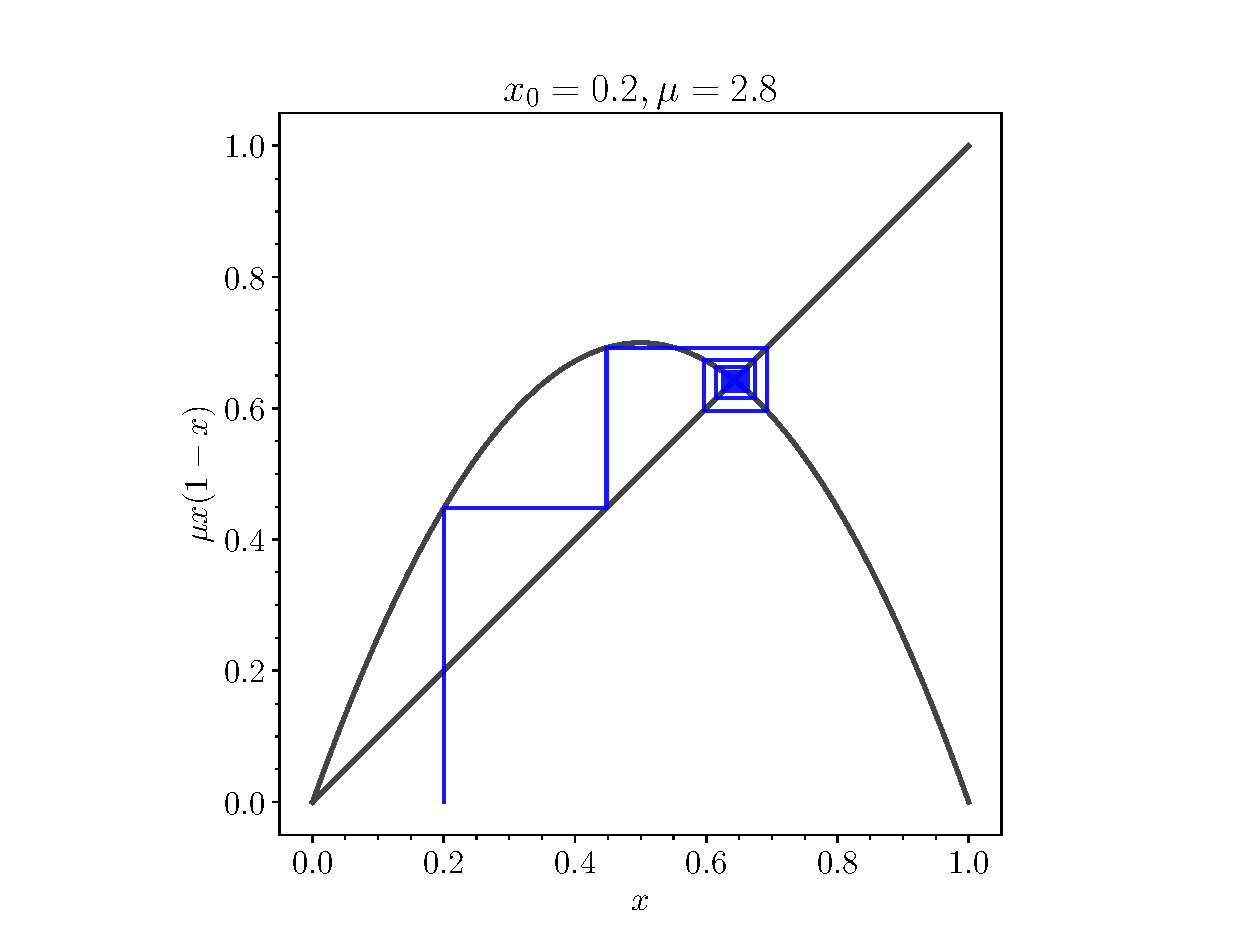
\includegraphics[scale=0.6]{cobweb_0.2_2.8}
\end{center}
\end{figure}

\begin{figure}
\begin{center}
\caption{Diagrama Cobweb de la ecuación logística, con $x_0=0.2$, $\mu=3.8$.}
\label{fig: cobweb_3.8}
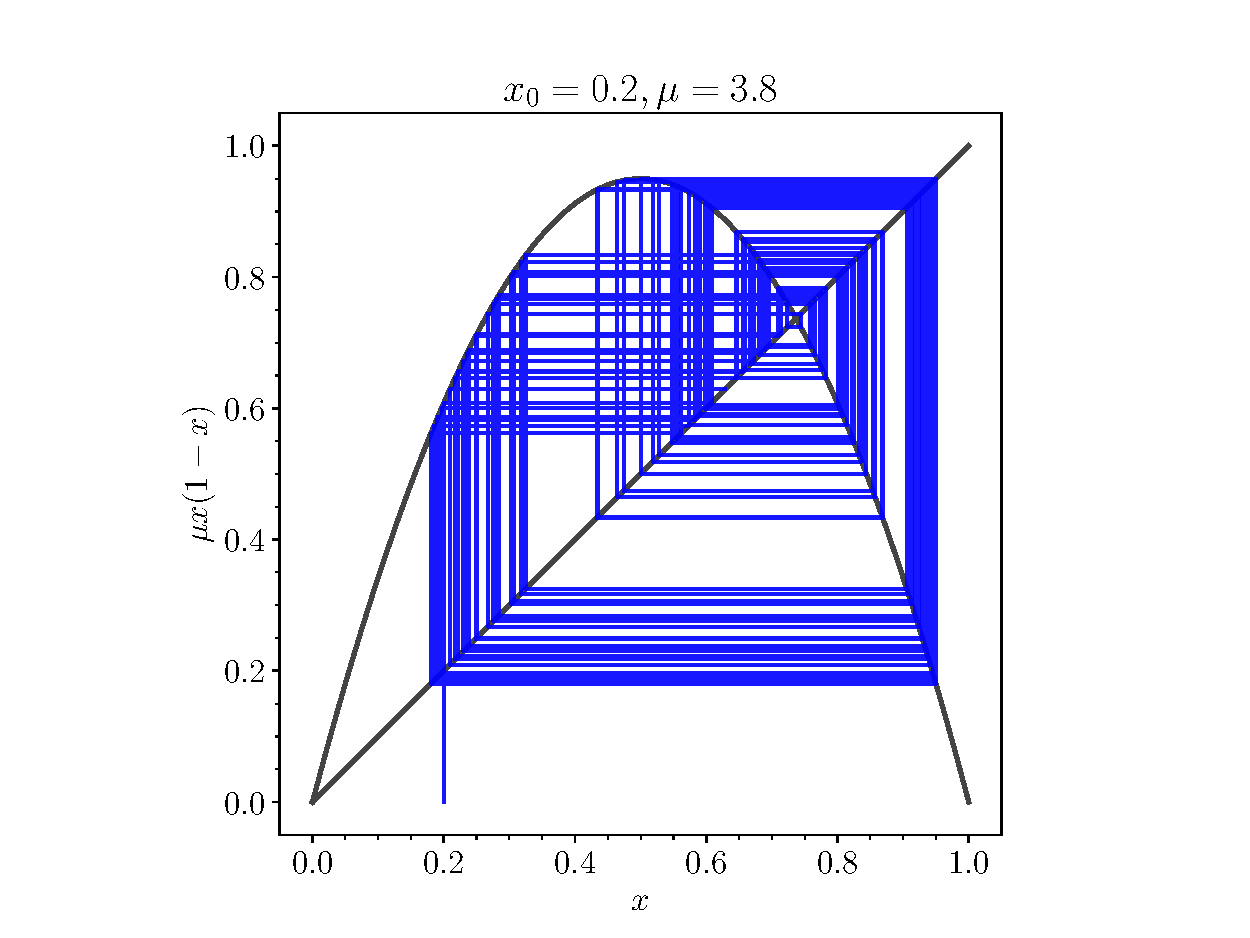
\includegraphics[scale=0.6]{cobweb_0.2_3.8}
\end{center}
\end{figure}

En \eqref{fig: cobweb_2.8} podemos ver como el punto de equilibrio $X^*=0$ es inestable y como el otro punto de equilibrio $X^*$ es localmente asintóticamente estable.

Asimismo, en \eqref{fig: cobweb_3.8} observamos como ambos puntos de equilibrio son inestables.

\end{proof}

\begin{proposition}
La ecuación logística tiene un 2-ciclo para todo $\mu > 3$, es decir, existen dos puntos $p$ y $q$ tal que $f(p)=q$ y $f(q)=p$.
\end{proposition}

\begin{proof}
Tenemos que $f(p)=q$ y $f(q)=p$ es equivalente a $f(f(p))=p$ y $f(f(q))=q$, es decir, $p$ es un punto fijo al iterar dos veces la función dada.

Como $f(x)$ es una función polinómica de segundo grado, entonces $f(f(x))$ será de cuarto grado, luego tendrá 4 raíces entre reales y complejas.

Por tanto necesitamos resolver la ecuación de cuarto grado $f(f(x))=x$. Sabemos que los puntos fijos de la ecuación logística cumplen $f(X^*)=X^*$, luego
$$f(f(X^*))=f(X^*)=X^*,$$
por lo que son solución de la ecuación. Y al factorizar conociendo estas soluciones el problema se reduce a resolver una ecuación cuadrática de la que obtenemos las siguientes raíces:
$$p,q=\frac{\mu+1\pm \sqrt{(\mu -3)(\mu +1)}}{2\mu}.$$

Estas soluciones son reales si $\mu > 3$ luego existe un 2-ciclo.

Si $\mu = 3$ estas raíces coinciden y valen $p=q=\frac{2}{3}=1-\frac{1}{3}=1-\frac{1}{\mu }$, luego no existe un 2-ciclo, hemos obtenido el mismo punto fijo.

Por último, si $\mu < 3$ las raíces no son reales y por tanto no existe un 2-ciclo.
\end{proof}

Si $\mu = 3.3$ tenemos  que la solución de la ecuación logística oscila repitiéndose cada dos iteraciones, es decir, sigue un 2-ciclo. Si $\mu = 3.5$ la solución se repite cada 4 iteraciones, luego sigue un 4-ciclo.
Se encuentran períodos más grandes (de 8, 16, 32...) a medida que $\mu$ toma valores mayores.

Sea $\mu_n$ el valor de $\mu$ para el cual aparece un $2^n$-ciclo. Entonces experimentalmente se obtiene que $\mu_n$ converge a un valor $\mu_\infty=3.569946...$.


\begin{proposition}
En la ecuación logística, se tiene que su solución converge si $\mu < 3$, oscila si $3 < \mu \lesssim 3.57$ y se produce caos si $\mu \gtrsim 3.57$. 
\end{proposition}


\section{Epidemiología}

Las enfermedades infecciosas como la influenza (o gripe) o la tuberculosis pueden ser severas. La epidemia del SIDA, pandemias recurrentes de influenza, brotes de ébola y la pandemia del Covid-19 son acontecimientos que preocupan e interesan a muchas personas. La prevalencia y los efectos de estas enfermedades sobre todo en países menos desarrollados son menos estudiadas, pero de mayor interés, pues la mortalidad de estas y otras enfermedades en estas zonas es mucho mayor que en países desarrollados. Muchas enfermedades como la malaria o el cólera son endémicas en muchas partes del mundo. Los efectos de enfermedades con alta mortalidad en la esperanza de vida y en la economía de los países afectados es considerable. Por ello, el estudio y modelado de epidemias es muy relevante.

A continuación se explican algunos conceptos básicos de epidemiología. Para esta sección se ha usado principalmente \cite{brauerMathematicalModelsPopulation2012}

\begin{definition}
Las epidemias son brotes espontáneos de una enfermedad o situaciones endémicas, en las que la enfermedad está siempre presente.
\end{definition}

Los individuos de una población se pueden dividir en tres grupos, haciendo referencia a su situación con respecto a la enfermedad.

\begin{definition}
Los individuos susceptibles, que denotamos $S_n$, son aquellos que pueden infectarse con la enfermedad pero aún no lo han hecho en el momento $n$.
\end{definition}

\begin{definition}
Los individuos infectados, a los que denotamos $I_n$, son las personas infectadas en el instante $n$ por la enfermedad y pueden contagiar la enfermedad a los individuos susceptibles.
\end{definition}

\begin{definition}
Los individuos recuperados, que denotamos $R_n$, son los individuos que han estado infectados y ya no contagian la enfermedad ni pueden volver a infectarse.
Los individuos recuperados hacen referencia a los individuos inmunizados, aislados, recuperados o fallecidos.
\end{definition}

\section{Tipos de modelos}

Los modelos discretos (principalmente SI, SIR y SIS) usan los estados Susceptible, Infectado y Recuperado. Los nombres suelen hacer referencia al flujo que se sigue para pasar entre los estados. Así, por ejemplo un modelo SI pasa de susceptible a infectado, uno SIR de susceptible a infectado y recuperado y SIS alterna entre susceptible e infectado.

En estos modelos se hacen dos suposiciones:
\begin{enumerate}
\item La población se mezcla de manera homogénea, es decir, todos los individuos tienen la misma probabilidad de contraer la enfermedad.
\item El total de la población es constante y lo denotaremos por $N$.
\end{enumerate}

